\documentclass[a4papper]{article}

\usepackage[final]{pdfpages}
\usepackage{graphicx}
\usepackage{amssymb, amsmath, amsthm, mathrsfs}
\usepackage{indentfirst}
\usepackage{amsmath}
\newtheoremstyle{neosn}{0.5\topsep}{0.5\topsep}{\rm}{}{\sc}{.}{ }{\thmname{#1}\thmnumber{ #2}\thmnote{ {\mdseries#3}}}
\theoremstyle{neosn}
\newtheorem{problem}{Problem}

\begin{document}
    \begin{center}
        {\bf Homework 1 of Lexture Computational Complexity}\\
        \today \\
        Tanglin
    \end{center}

    \problem{Construct a single-tape Turing Machine, which can find
    out which number is greater than the other for two n-bits natural numbers $x,y$
    in time $O(n^2)$.}\\

    Solution:\\

    By the definition of Turing Machine, let alphabet symbol set
    \[
        A = \{0,1,S,M,\Lambda,X,\text{Less},\text{Greater},\text{Equal}\}
    \]
    and status set
    \[
        Q = \{q_0, q_1, r_s, r_0, r_1, r_{00}, r_{11},
        f_e,f_{ee}, f\}
    \]
    where $q_0$ is the initial status, $f$ the final status.\\

    First, let me show how we should set the tape in order to calculate
    this problem.\\

    \begin{figure}[h]
        \centering
        \begin{tabular}{|c|c|c|c|c|c|c|c|c|c|c|c|c|c|c|c|c|c|}
            \hline
            \cdots & \Lambda & \Lambda & \Lambda &
            S & b & b & \cdots & b & M & b & b &
            \cdots& b & \Lambda & \Lambda & \cdots \\
            \hline
        \end{tabular}\caption{The tape with initial cell S, where b is 0 or 1.}
        \label{fig:figure}
    \end{figure}

    The second cell to the left of S is result bit, and cell S is the initial cell. \\

    It is necessary to explain elements of the alphabet set: \\
    \[
    \begin{array}{lll}
        0 & \text{---} & \text{the binary number 0.}\\
        1 & \text{---} & \text{the binary number 1.}\\
        \Lambda & \text{---} & \text{the empty symbol.}\\
        S & \text{---} & \text{the initial position.}\\
        M & \text{---} & \text{the separate symbol which distinguishes two binary numbers.}\\
        X & \text{---} & \text{the symbol denotes that the bit was extracted.}\\
        \text{Greater} & \text{---} & \text{result symbol denotes the first number is greater.}\\
        \text{Less} & \text{---} & \text{result symbol denotes the first number is less.}\\
        \text{Equal} & \text{---} & \text{result symbol denotes the two numbers are equal.}\\
    \end{array}
    \] \\

    The statuses are difficult to explain in detail, I will show the transposition table, and the transposition graph to help us understand it.
    I can only little explain some of them, $q_0$ is the initial status, $r_s$ means the head prepare to get the highest bit of a number(the first or the second),
    $r_0$ or $r_1$ means that the head get the bit $0$ or $1$ and then it will set the bit to X and skip all the cell until meets $\Lambda$, then it changes to status
    $r_{00}$ or $r_{11}$, then it go to the left cell and set the bit if the cell with $\Lambda$, or it compares the bit with information in head, if the cell is $\Lambda$,
    it denotes that this head got bit from the first number, then the status changes to $q_1$ which means the head will go and get the corresponding bit of the second number, or
    a new loop will start. The status $f_e$ and $f_{ee}$ used to deal with the case that two numbers are equal.\\

    This is the transposition table, in other words, the function
    \[
        \delta: A \times Q \to A \times Q \times \{-1, 0, 1\}
    \]
    I will give the full map:
    \begin{enumerate}
        \item Start from the initial cell with initial status $q_0$.
        \[
            (S, q_0) \mapsto (S, r_s, 1)
        \]
        \item Get the last unextracted bit of the first number and set it to X, then
        send it to the result bit.
        \[
            \begin{array}{lll}
            (0, r_s) \mapsto (X, r_0, -1) & (1, r_s) \mapsto (X, r_1, -1) & (X, r_s) \mapsto (X, r_s, 1) \\
            (S, r_0) \mapsto (S, r_0, -1) & (X, r_0) \mapsto (X, r_0, -1) &  \\
            (S, r_1) \mapsto (S, r_1, -1) & (X, r_1) \mapsto (X, r_1, -1) & \\
            (\Lambda, r_0) \mapsto (\Lambda, r_{00}, -1) & (\Lambda, r_1) \mapsto (\Lambda, r_{11}, -1) & \\
            (\Lambda, r_{00}) \mapsto (0, q_1, 1) & (\Lambda, r_{11}) \mapsto (1, q_1, 1) & \\
            \end{array}
        \]
        \item Get the last unextracted bit of the second number and set it X,
        then send the information to the result bit.
        \[
            \begin{array}{ll}
            (\Lambda, q_1) \mapsto (\Lambda, q_1, 1) & (S, q_1) \mapsto (S, q_1, 1) \\
            (0, q_1) \mapsto (0, q_1, 1) & (1, q_1) \mapsto (1, q_1, 1) \\
            (X, q_1) \mapsto (X, q_1, 1) & \\
            (M, q_1) \mapsto (M, r_s, 1) & \\
            (M, r_0) \mapsto (M, r_0, -1) & (M, r_1) \mapsto (M, r_1, -1) \\
            (0, r_0) \mapsto (0, r_0, -1) & (0, r_1) \mapsto (0, r_1, -1) \\
            (1, r_0) \mapsto (1, r_0, -1) & (1, r_1) \mapsto (1, r_1, -1) \\
            \end{array}
        \]
        \item Compare the two bits and halt when compare all the bits.
        \[
            \begin{array}{ll}
            (0, r_{00}) \mapsto (\Lambda, q_0 ,1) & (1, r_{11}) \mapsto (\Lambda, q_0, 1) \\
            (\Lambda, q_0) \mapsto (\Lambda, q_0, 1) & \\
            (0, r_{11}) \mapsto (\text{Less}, f, 0) & (1, r_{00}) \mapsto (\text{Greater}, f, 0) \\
            (M, r_s) \mapsto (M, f_e, -1) & (X, f_e) \mapsto (X, f_e, -1) \\
            (S, f_e) \mapsto (S, f_e, -1) & (\Lambda, f_e) \mapsto (\Lambda, f_{ee}, -1) \\
            (\Lambda, f_{ee}) \mapsto (\text{Equal}, f, 0) & \\
            \end{array}
        \]
    \end{enumerate}

    These are all, and then I give the graph.

    \includepdfset{pagecommand={\thispagestyle{fancy}}}
    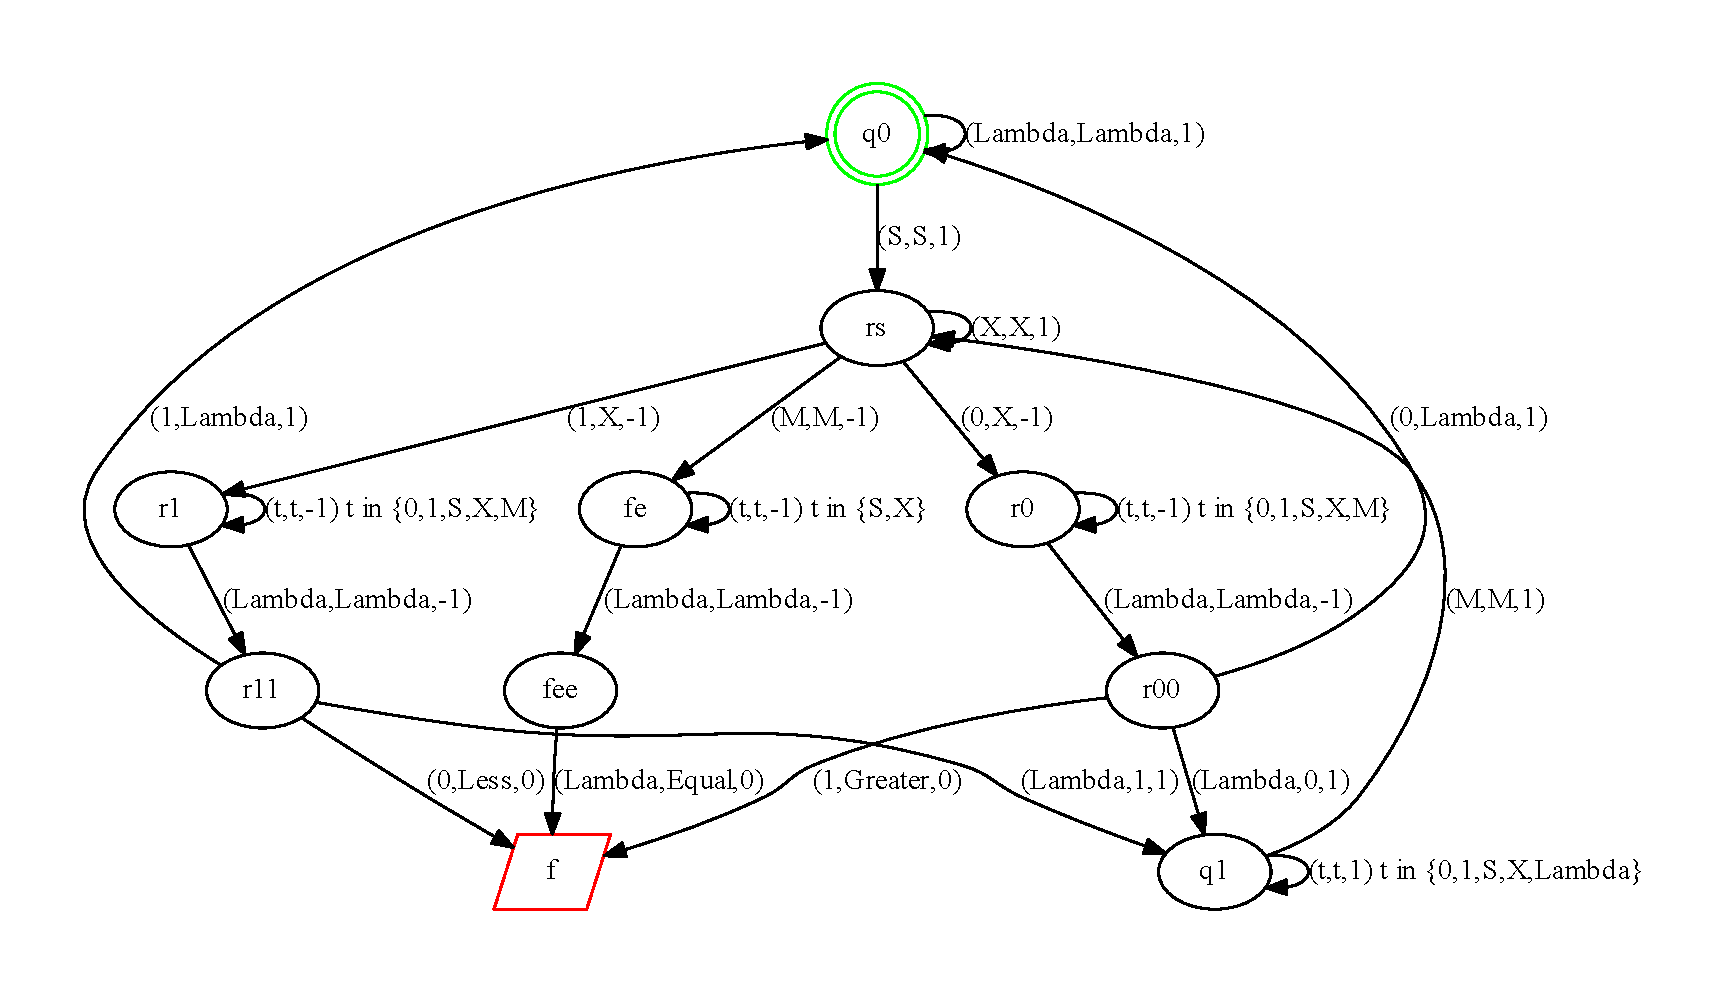
\includepdf{Comparator.gv.pdf}

    The arrow from one circle(status $p$) to another(status $q$)  with triple $(a,b,c \in \{-1,0,1\})$ means that,
    the head with status $p$ and the cell with content $a$, it will move to the left($c=-1$), right($c=1$) or stay($c=0$),
    and change the content $a$ to $b$. \\

    I have written a Python script to simulate this Turing Machine, and it will work well,
    the code in the attachment, you can test it with different inputs. \\
    \\

    \problem{Construct a single-tape Turing Machine, which can find
    out which sum of two n-bits natural numbers $x,y$
    in time $O(n^2)$.}\\

    Solution: \\

    I build a machine with 31 status, it is a little complex.
    The annotation you can find in the solution of the first problem.
    I just give the necessary explanation. \\

    The alphabet set and status set:
    \begin{gather*}
        A = \{0,1,X, \Lambda, R, M, S\} \\
        \\
        Q = \{q_0, g_r, r, r_g, r_{g1}, r_{g0},r_{g11}, r_{g00}, \\
        g_l, l, l_g,l_{g1}, l_{g0}, l_{g11}, l_{g00},l_{g0p}, l_{g1p}, l_p, l_{pp},\\
        r_f, f_f, f_{f0}, f_{f1}, f_1, f,\\
        0_{check_R}, 1_{check_R}, R_{set1}, R_{set0},\\
        0_{CR}, 1_{CR}\}\\
    \end{gather*}

    Where R means that cell on the left of R is used to store overflow bit.\\

    The tape is of form:

    \begin{figure}[h]
        \centering
        \begin{tabular}{|c|c|c|c|c|c|c|c|c|c|c|c|c|c|c|c|c|c|c|c|}
            \hline
            \cdots & \Lambda & 0 & R & \Lambda & \cdots & \Lambda &
            S & b & \cdots & b & M & b &
            \cdots& b & \Lambda & \cdots \\
            \hline
        \end{tabular}\caption{The tape with initial cell S, where b is 0 or 1.}
        \label{fig:figure1}
    \end{figure}

    It's worth noting that, we have to leave enough cells from R to S, because these cells are used
    to store result, in other words, if we find sum of two $n$-bits number, we have to leave at least
    $n+1$ cells between R and S\@.\\

    Before giving the transposition table and graph, I will explain these statues in brief.
    The status $q_0$ is the initial status, $g_r, r, r_g$ are the statuses for prepare to get
    the bit of the second number, $r_{g0}, r_{g1}$ denote that head get bit information $0$ or $1$,
    $r_{g00}, r_{g11}$ mean that the head has brought the information to result area, $g_l, l, l_g, l_{g0}, l_{g1},$
    $l_{g00}, l_{g11}$ are similar, they are for the first number. $l_{g0p}, l_{g1p}, l_p, l_{pp}$ are used to deal with
    set overflow bit, $0_{check_R}, 1_{check_R}, R_{set0}, R_{set1}, 1_{CR}, 0_{CR}$ are used to deal with overflow bit when
    new bit comes. $r_f, f_f, f_{f0}, f_{f1}, f_1, f$ are used to deal with the final case and halt. \\

    There are the transposition table:

    \begin{enumerate}
        \item Start from initial cell with initial status.
        \[
            \begin{array}{ll}
            (S, q_{0}) \mapsto (S, g_{r}, 1) & (1, g_{r}) \mapsto (1, g_{r}, 1) \\
            (0, g_{r}) \mapsto (0, g_{r}, 1) & (M, g_{r}) \mapsto (M, r, 1) \\
            (1, r) \mapsto (1, r, 1) & (0, r) \mapsto (0, r, 1) \\
            (\Lambda, r) \mapsto (\Lambda, r_{g}, -1) & (X, r) \mapsto (X, r_{g}, -1)\\
            \end{array}
        \]
        \item Get the first bit of the rest bits of the second number, and set it to X.
        \[
            \begin{array}{ll}
            (1, r_{g}) \mapsto (X, r_{g1}, -1) & (0, r_{g}) \mapsto (X, r_{g0}, -1) \\
            \end{array}
        \]
        \item Skip the other bits.
        \[
            (p, q) \mapsto (p, q, -1), \text{where } p \in \{1,0,X,M,S\}, q \in \{r_{g1}, r_{g0}\}.
        \]
        \item Set the corresponding bit by information of head.
        \[
            \begin{array}{ll}
                (\Lambda, r_{g0}) \mapsto (\Lambda, r_{g00}, -1) & (\Lambda, r_{g1}) \mapsto (\Lambda, r_{g11}, -1) \\
                (\Lambda, r_{g00}) \mapsto (0, 0_{_check_R}, -1) & (\Lambda, r_{g11}) \mapsto (1, 1_{_check_R}, -1) \\
            \end{array}
        \]
        \item Skip set bit till Lambda while present status with $r_{g00}$ or $r_{g11}$.
        \[
            (p, q) \mapsto (p, q, -1), \text{where } p \in \{0,1\}, q \in \{r_{g00}, r_{g11}\}.
        \]
        \item Skip all alphabet till 'R' while present status is $0_{check_R}$ or $1_{check_R}$.
        \[
            (p, q) \mapsto (p, q, -1), \text{where } p \in \{0, 1, \Lambda\}, q \in \{0_{check_R}, 1_{check_R}\}.
        \]
        \item Check overflow and handle these cases.
        \[
            \begin{array}{ll}
                (R, 0_{check_R}) \mapsto (R, 0_{CR}, -1) & (R, 1_{check_R}) \mapsto (R, 1_{CR}, -1) \\
                (0, 0_{CR}) \mapsto (0, g_{l}, 1) & (0, 1_{CR}) \mapsto (0, g_{l}, 1) \\
                (1, 0_{CR}) \mapsto (0, R_{set1}, 1) & (1, 1_{CR}) \mapsto (1, R_{set0}, 1)\\
                (\Lambda, R_{set0}) \mapsto (\Lambda, R_{set0}, 1) & (\Lambda, R_{set1}) \mapsto (\Lambda, R_{set1}, 1) \\
                (R, R_{set0}) \mapsto (R, R_{set0}, 1) & (R, R_{set1}) \mapsto (R, R_{set1}, 1)\\
                (0, R_{set0}) \mapsto (0, g_{l}, 1) & (0, R_{set1}) \mapsto (1, g_{l}, 1) \\
                (1, R_{set0}) \mapsto (0, g_{l}, 1) & (1, R_{set1}) \mapsto (1, g_{l}, 1) \\
                (0, r_{g00}) \mapsto (0, r_{g00}, -1) & (1, r_{g00}) \mapsto (1, r_{g00}, -1) \\
                (R, r_{g00}) \mapsto (1, g_{l}, 1) & \\
            \end{array}
        \]
        \item Go back to the initial cell and prepare to get the corresponding bit in the first number.
        \[
            (p, g_l) \mapsto (p, g_l, 1), \text{where } p \in \{0,1,\Lambda,R\}.
        \]
        \item To get the corresponding bit of the first number.
        \[
            \begin{array}{ll}
                (S, g_{l}) \mapsto (S, l, 1) & (1, l) \mapsto (1, l, 1) \\
                (0, l) \mapsto (0, l, 1) & (M, l) \mapsto (M, l_{g}, -1) \\
                (X, l) \mapsto (X, l_{g}, -1) & \\
                (1, l_{g}) \mapsto (X, l_{g1}, -1) & (0, l_{g}) \mapsto (X, l_{g0}, -1)\\
            \end{array} \\

            (p, q) \mapsto (p, q, -1), \text{where } p \in \{1,0,S\}, q \in \{l_{g1}, l_{g0}\}.
        \]
        \item Put the bit we got to the result bits and handle some cases.
        \[
            \begin{array}{ll}
                (\Lambda, l_{g1}) \mapsto (\Lambda, l_{g11}, -1) & (\Lambda, l_{g0}) \mapsto (\Lambda, l_{g00}, -1) \\
            \end{array}
        \]
        \item Skip the last bits.
        \[
            (p,q) \mapsto (p, q, -1), \text{where } p \in \{0,1\}, q \in \{l_{g00}, l_{g11}\}.
        \]
        \item Handling these cases.
        \[
            \begin{array}{ll}
                (\Lambda, l_{g00}) \mapsto (\Lambda, l_{g0p}, 1) & (\Lambda, l_{g11}) \mapsto (\Lambda, l_{g1p}, 1) \\
                (0, l_{g0p}) \mapsto (0, q_{0}, 1) & (0, l_{g1p}) \mapsto (1, q_{0}, 1) \\
                (1, l_{g0p}) \mapsto (1, q_{0}, 1) & (1, l_{g1p}) \mapsto (0, l_{p}, -1) \\
                (\Lambda, l_{p}) \mapsto (\Lambda, l_{p}, -1) & (R, l_{p}) \mapsto (R, l_{pp}, -1) \\
                (0, l_{pp}) \mapsto (1, q_{0}, 1) & \\
            \end{array}
        \]
        \item Go back to the initial position and execute the next bit.
        \[
            (p, q_0) \mapsto (p ,q_0, 1), \text{where } p \in \{0,1,\Lambda, R\}.
        \]
        \item When we handle all the bits, then halt.
        \[
            \begin{array}{ll}
                (X, g_{r}) \mapsto (X, g_{r}, 1) & (M, r_{g}) \mapsto (M, r_{f}, -1) \\
            \end{array} \\

            (p, r_f) \mapsto (p, r_f, -1), \text{where } p \in \{0,1,X,S,\Lambda\}.

            \begin{array}{ll}
                (R, r_{f}) \mapsto (R, f_{f}, -1) & (0, f_{f}) \mapsto (0, f_{f0}, 1) \\
                (1, f_{f}) \mapsto (0, f_{f1}, 1) & \\
            \end{array} \\

            (p, q) \mapsto (p ,q, 1), \text{where } p \in \{\Lambda, R\}, q \in \{f_{f0}, f_{f1}\}.

            \begin{array}{ll}
                (0, f_{f0}) \mapsto (0, f, 0) & (1, f_{f0}) \mapsto (1, f, 0) \\
                (0, f_{f1}) \mapsto (0, f_{1}, -1) & (\Lambda, f_{1}) \mapsto (1, f, 0) \\
                (1, f_{f1}) \mapsto (1, f_{1}, -1) & \\
            \end{array}
        \]
    \end{enumerate}

    And then the transposition graph.
    \includepdfset{pagecommand={\thispagestyle{fancy}}}
    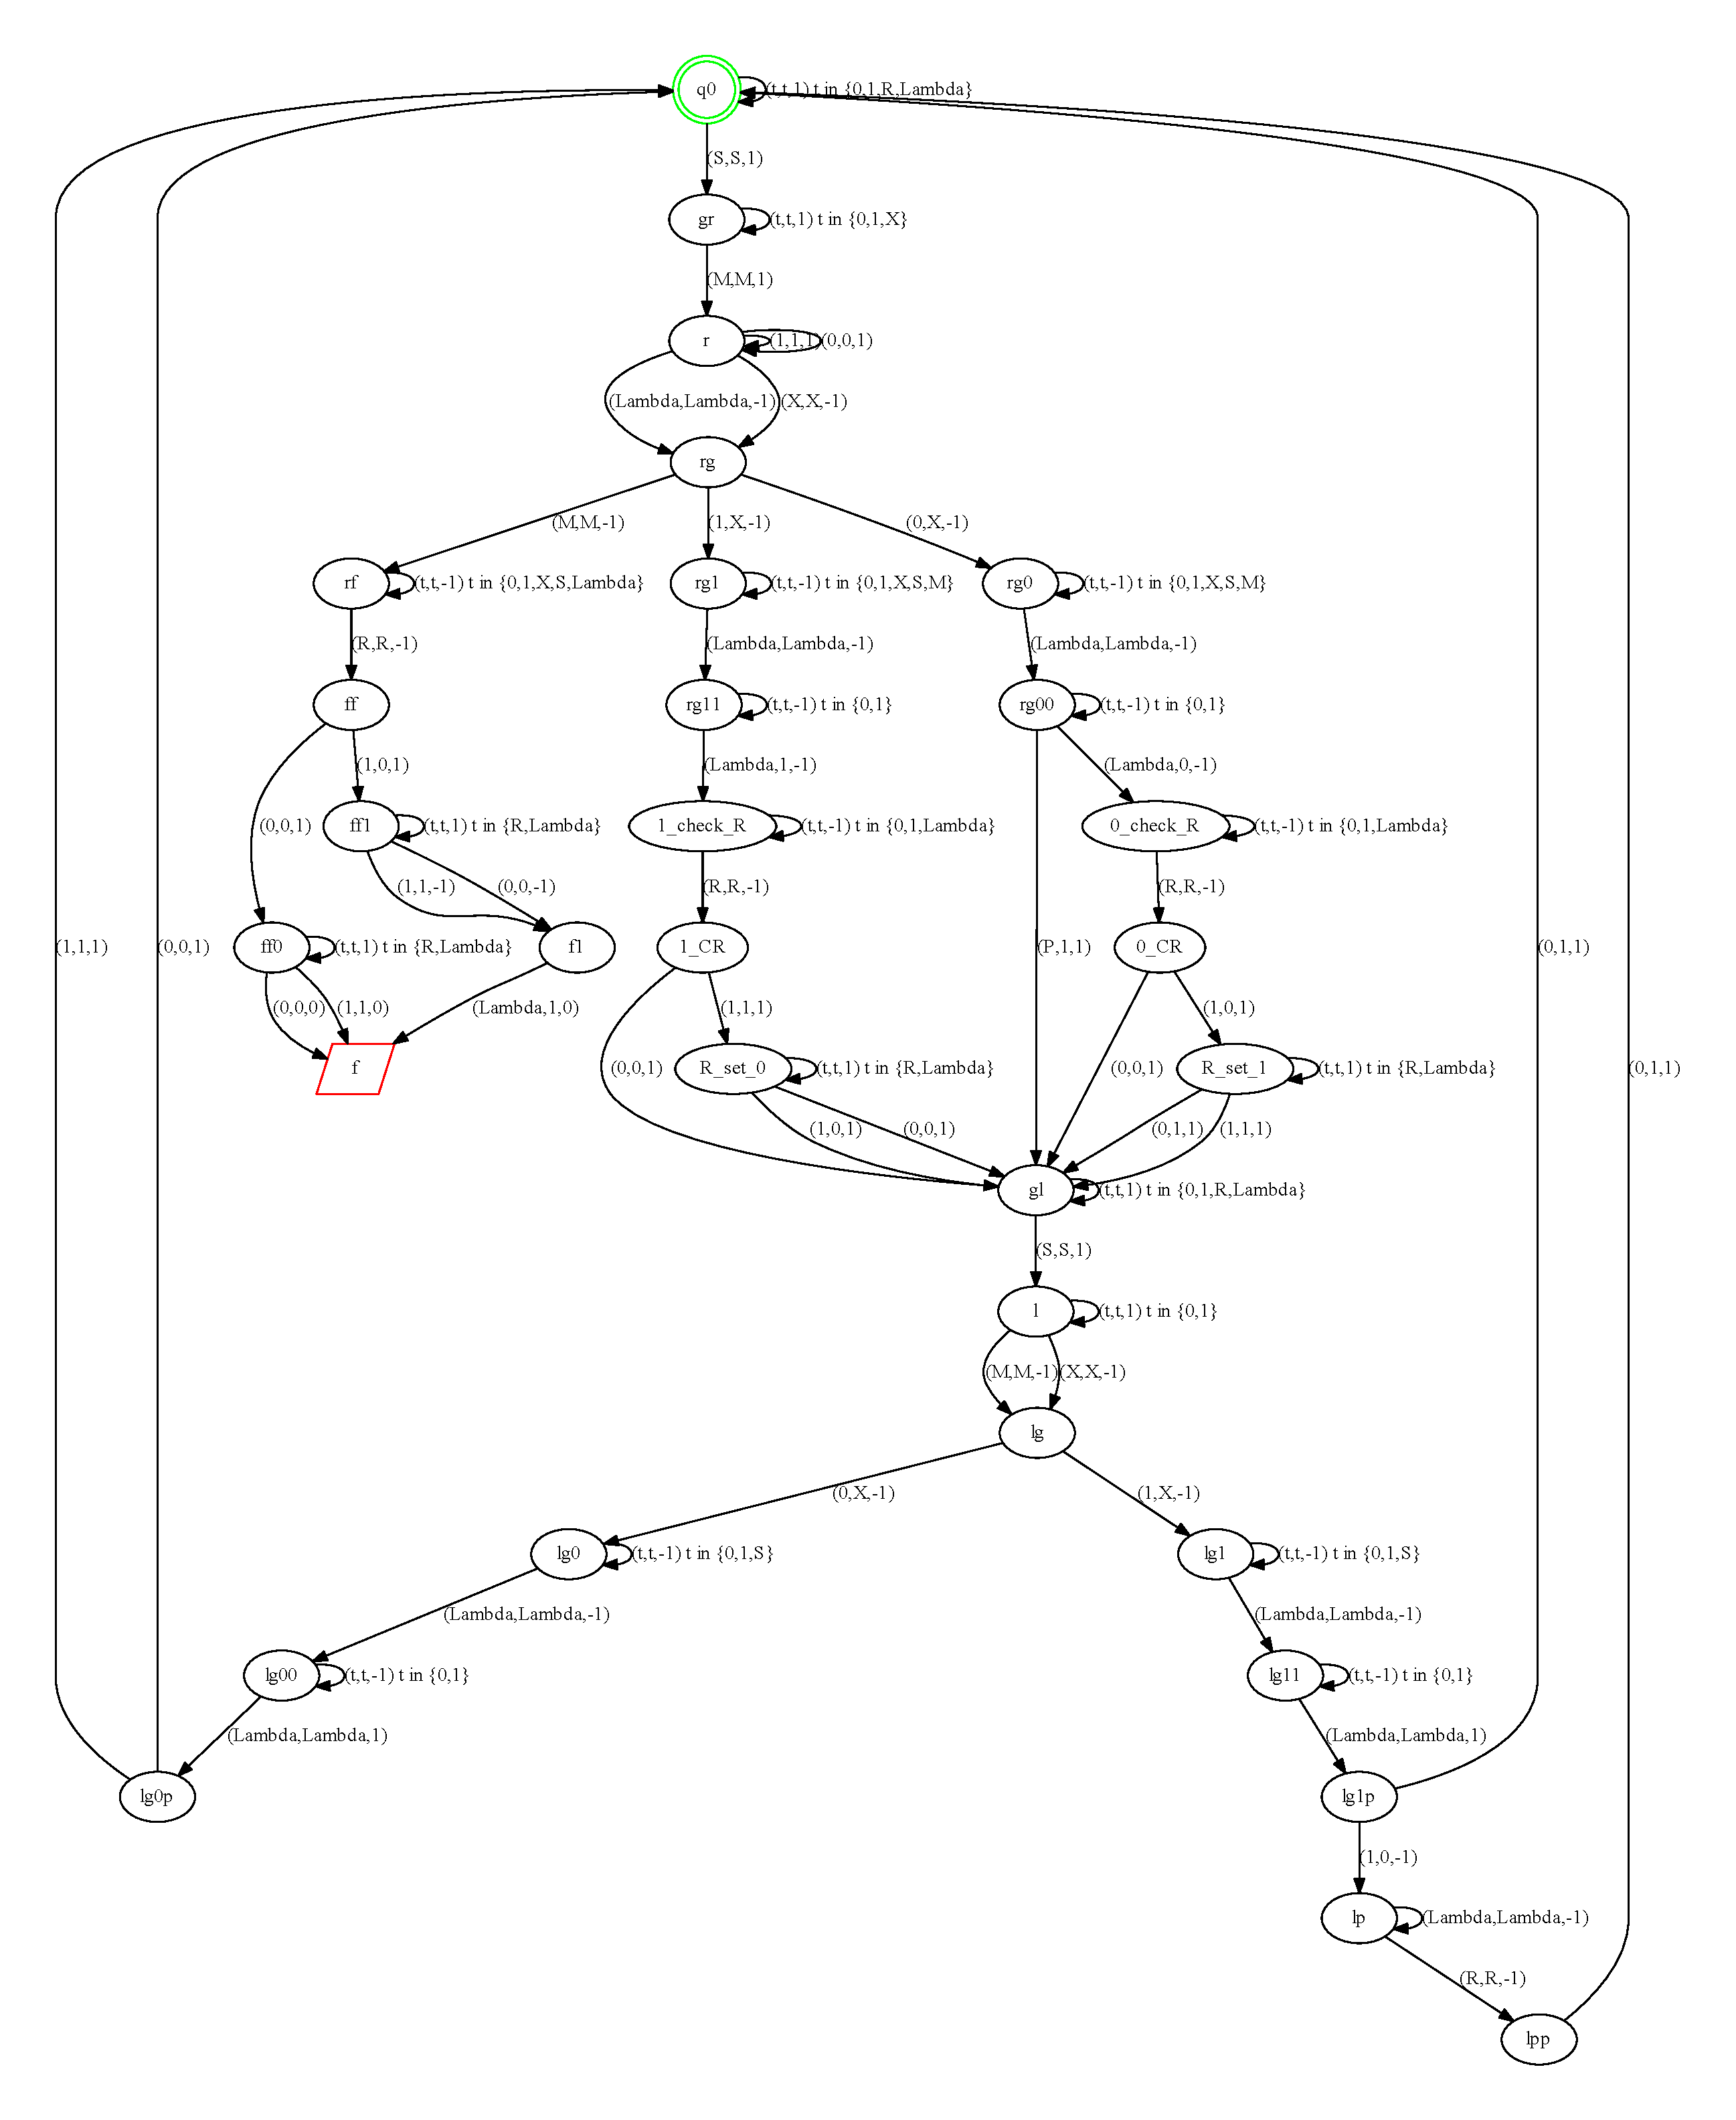
\includepdf{Adder.gv.pdf}

    I also write a simulation for this Adder Turing machine, you can find it in the attachment and
    test it.
    It works well.
\end{document}